%------------------------------------------------------------
%------------------------------------------------------------


\begin{frame}
\frametitle{The U Rune Exercise}
\begin{columns}[c] % The "c" option specifies centered vertical alignment while the "t" option is used for top vertical alignment

\column{.37\textwidth} % Left column and width
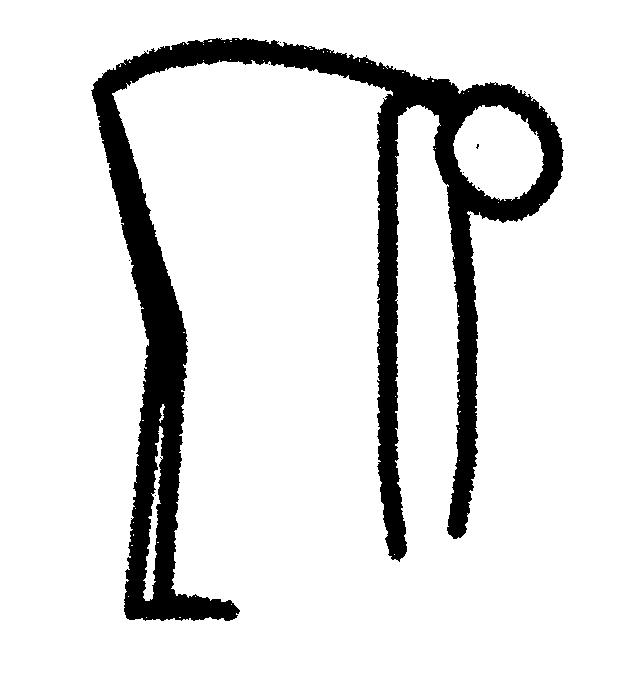
\includegraphics[width=\linewidth]{ExerciseU.png}

\column{.4\textwidth} % Right column and width
\structure{Bend over, reach down}, arms and fingertips pointing to the ground.

\vspace{5mm}
\structure{Rooting}. 

Creates the \structure{ground for powerful actions}.

\vspace{5mm}
Activates the \structure{nervous center in the head}.
\column{.29\textwidth} % Right column and width

\includegraphics[width=\linewidth]{RuneU.png}
\end{columns}

\end{frame}
%------------------------------------------------------------
%------------------------------------------------------------

\begin{frame}
\frametitle{The I Rune Exercise}
\begin{columns}[c] % The "c" option specifies centered vertical alignment while the "t" option is used for top vertical alignment

\column{.2\textwidth} % Left column and width
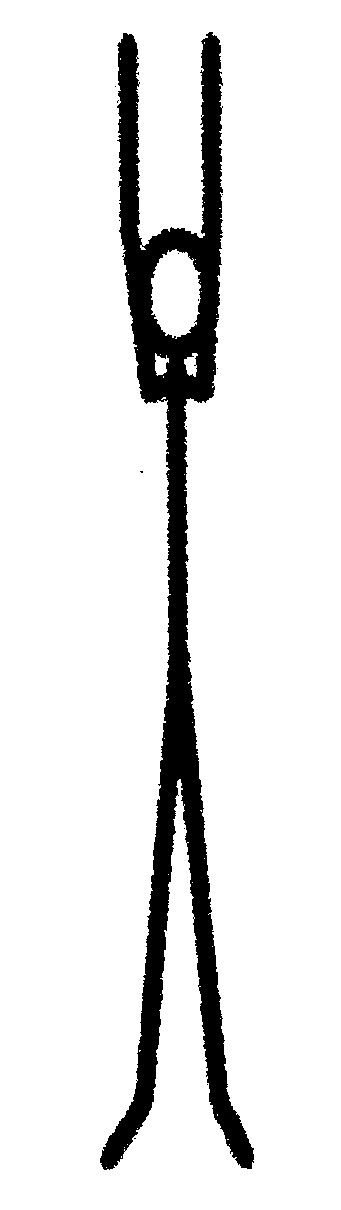
\includegraphics[width=\linewidth]{ExerciseI.png}

\column{.4\textwidth} % Right column and width
\structure{Stand upright}, face forward; hold arms vertical, \structure{hands touching high above the head}. 

\vspace{5mm}
\structure{Clarity of mind}.

Patience.

Danger of hardening.

\vspace{5mm}
\structure{Relaxation of the muscles}.
\column{.26\textwidth} % Right column and width

\includegraphics[width=\linewidth]{RuneI.png}
\end{columns}

\end{frame}
%------------------------------------------------------------
%------------------------------------------------------------


\begin{frame}
\frametitle{The Y Rune Exercise}
\begin{columns}[c] % The "c" option specifies centered vertical alignment while the "t" option is used for top vertical alignment

\column{.37\textwidth} % Left column and width
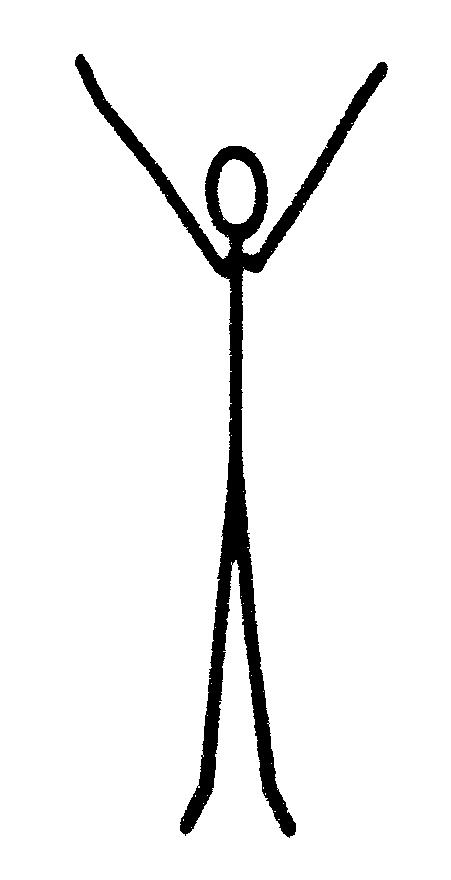
\includegraphics[width=\linewidth]{ExerciseY.png}

\column{.3\textwidth} % Right column and width
Stand upright, face forward; \structure{hold arms at a 45\degree upwards, palms up}. 

\vspace{5mm}
\structure{Set the goal and let it ripen} in a sheltered place.

\vspace{5mm}
Transformation of the sexual energy.
\column{.42\textwidth} % Right column and width

\includegraphics[width=\linewidth]{RuneY.png}
\end{columns}

\end{frame}
%------------------------------------------------------------
%------------------------------------------------------------



\begin{frame}
\frametitle{The F Rune Exercise}
\begin{columns}[c] % The "c" option specifies centered vertical alignment while the "t" option is used for top vertical alignment

\column{.37\textwidth} % Left column and width
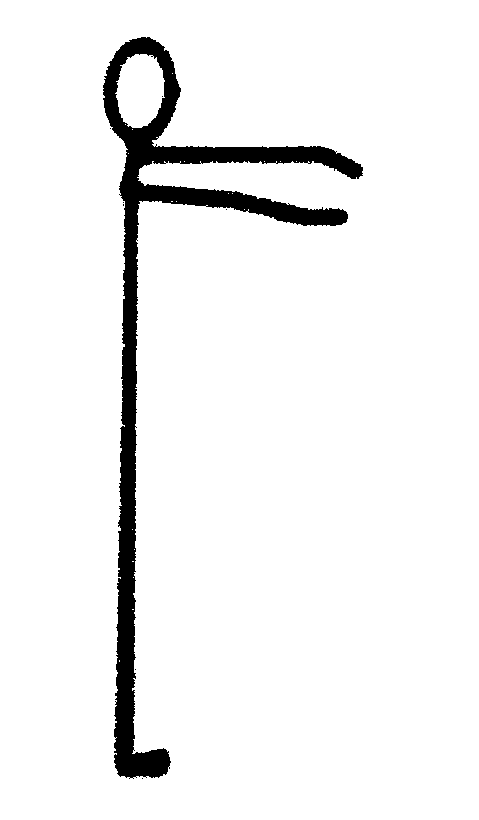
\includegraphics[width=\linewidth]{ExerciseF.png}

\column{.45\textwidth} % Right column and width
Stand upright, face forward; hold \structure{arms in front of you}, right hand on top of left hand. the middle and ring finger of each hand are bend and held with the thumbs as if you would be \structure{gripping an invisible broom stick} with both hands, \structure{pinkies and indices are stretched} straight.

The \structure{base of each new start}.

\vspace{5mm}
Solves energy bloackages.
\column{.37\textwidth} % Right column and width
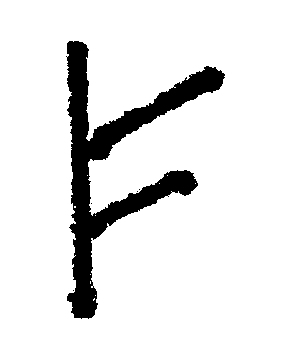
\includegraphics[width=\linewidth]{RuneF.png}
\end{columns}

\end{frame}
%------------------------------------------------------------
%------------------------------------------------------------



\begin{frame}
\frametitle{The T Rune Exercise}
\begin{columns}[c] % The "c" option specifies centered vertical alignment while the "t" option is used for top vertical alignment

\column{.41\textwidth} % Left column and width
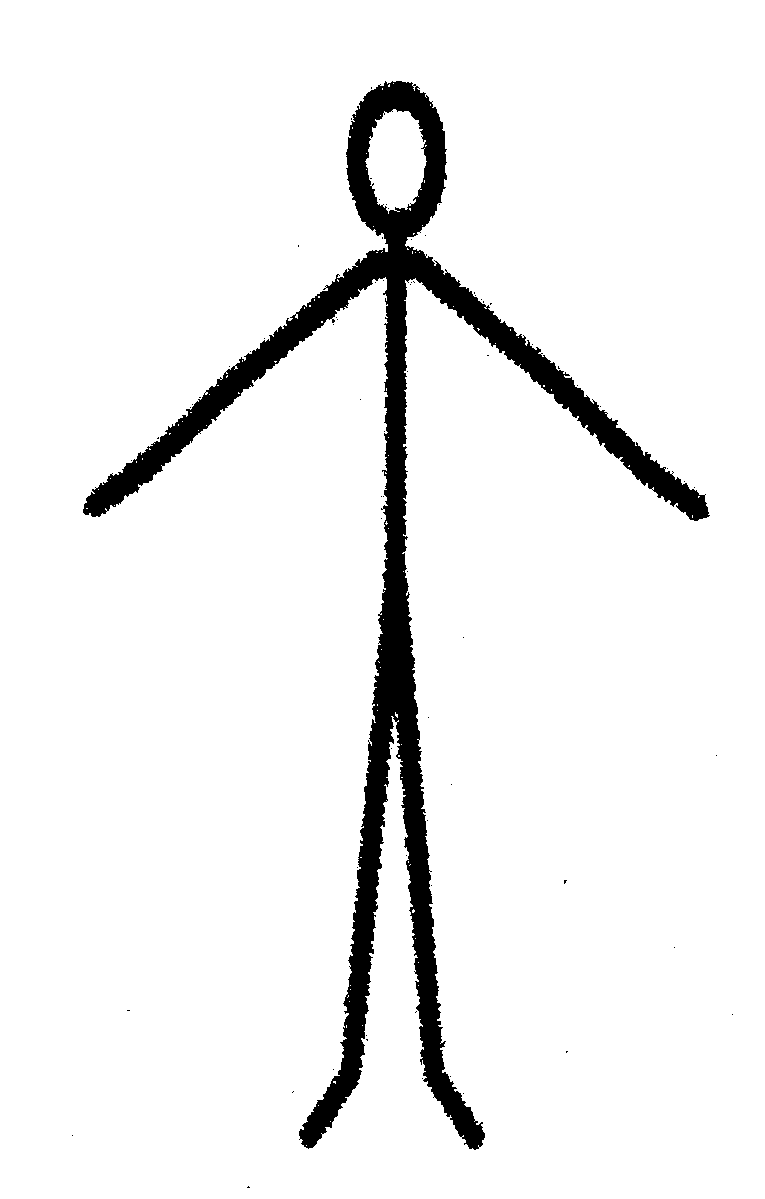
\includegraphics[width=\linewidth]{ExerciseT.png}

\column{.3\textwidth} % Right column and width
Stand upright, face forward, \structure{arms slanted down to the sides by 30\degree, palms downwards}.

\vspace{5mm}
\structure{Goal orientation}, to put a plan in action, realize.

\vspace{5mm}
Relaxes the muscles.

\structure{Activates the glands and the solar plexus}.
\column{.44\textwidth} % Right column and width
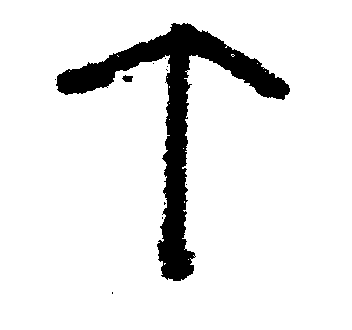
\includegraphics[width=\linewidth]{RuneT.png}
\end{columns}

\end{frame}
%------------------------------------------------------------
%------------------------------------------------------------

\begin{frame}
\frametitle{The W Rune Exercise -- instructions}
\begin{columns}[c] % The "c" option specifies centered vertical alignment while the "t" option is used for top vertical alignment

\column{.57\textwidth} % Left column and width
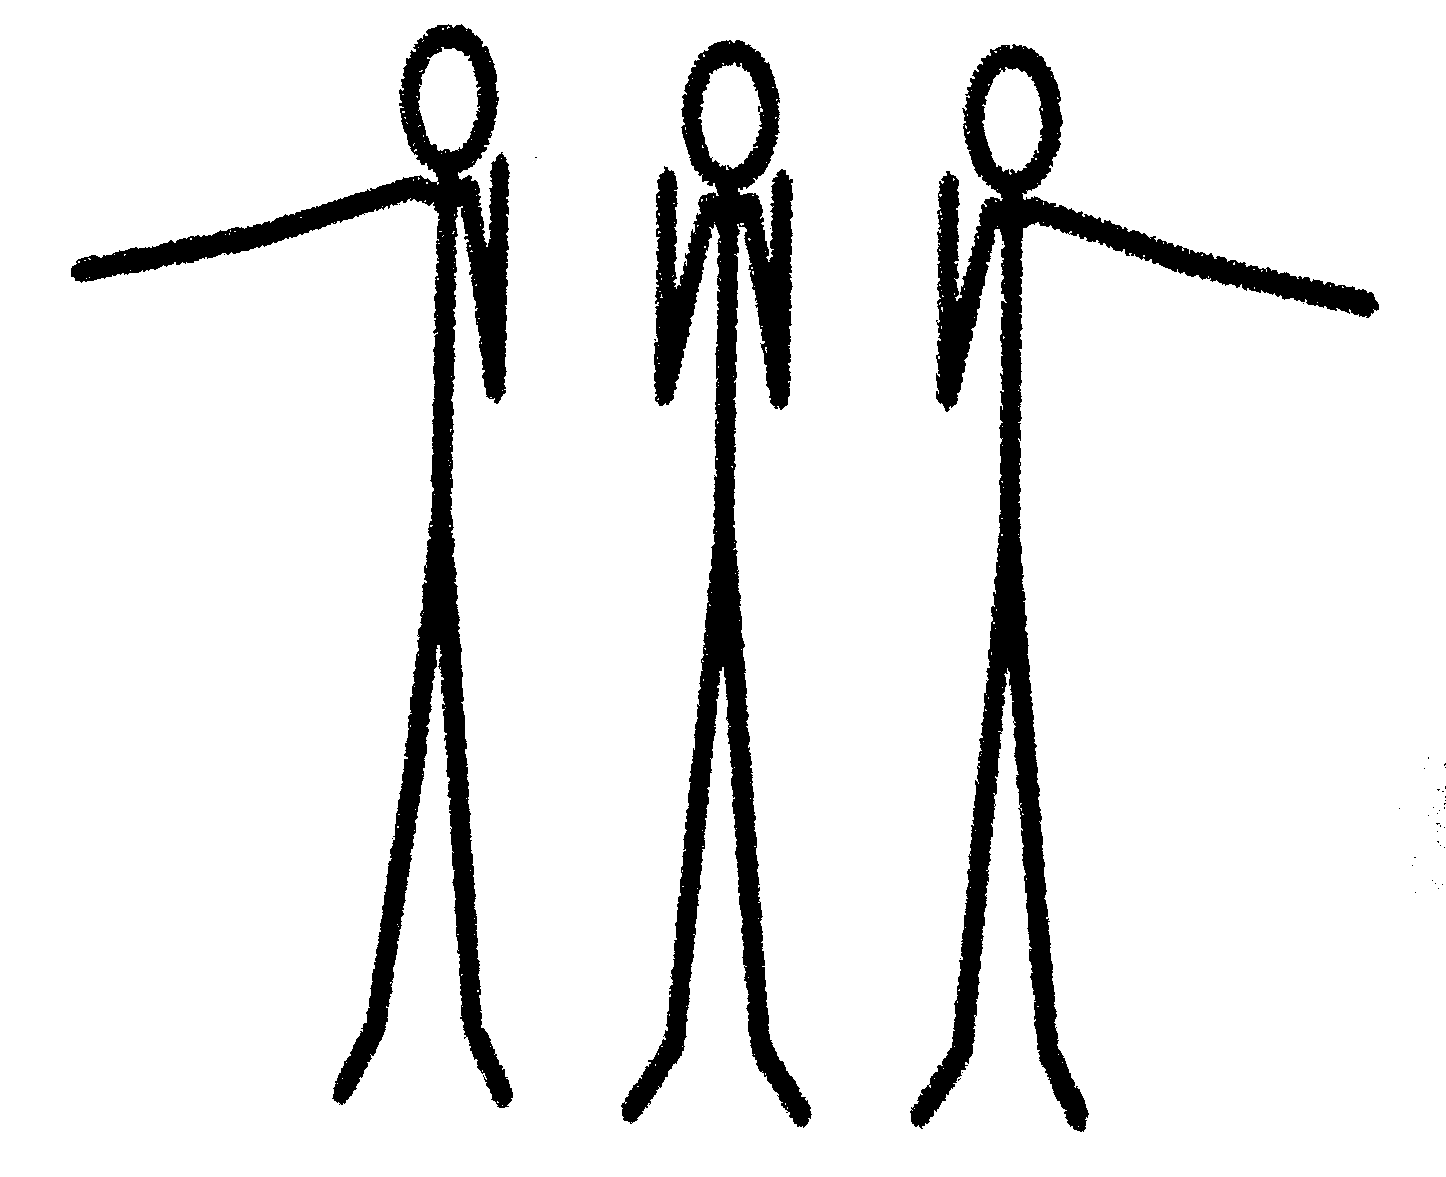
\includegraphics[width=\linewidth]{ExerciseW.png}

\column{.5\textwidth} % Right column and width
While standing, hold \structure{both arms in front of the chest}, \structure{parallel} with the edge of your hands facing forward.

\structure{Chop} with your \structure{right forearm} in an extension of the \structure{edge of your hand in a slicing motion} till you're in a \structure{horizontal position}, on the extension of your shoulder, while \structure{exhaling forcefully}. Like a \alert{karate chop}. \structure{Inhale while retrieving the arm} and then the same left. 

\structure{Repeat 15* each side}.


%\column{.24\textwidth} % Right column and width
%
\includegraphics[width=\linewidth]{RuneW.png}
\end{columns}

\end{frame}
%------------------------------------------------------------
%------------------------------------------------------------

%------------------------------------------------------------

\begin{frame}
\frametitle{The W Rune Exercise -- effects}
\begin{columns}[c] % The "c" option specifies centered vertical alignment while the "t" option is used for top vertical alignment

\column{.57\textwidth} % Left column and width
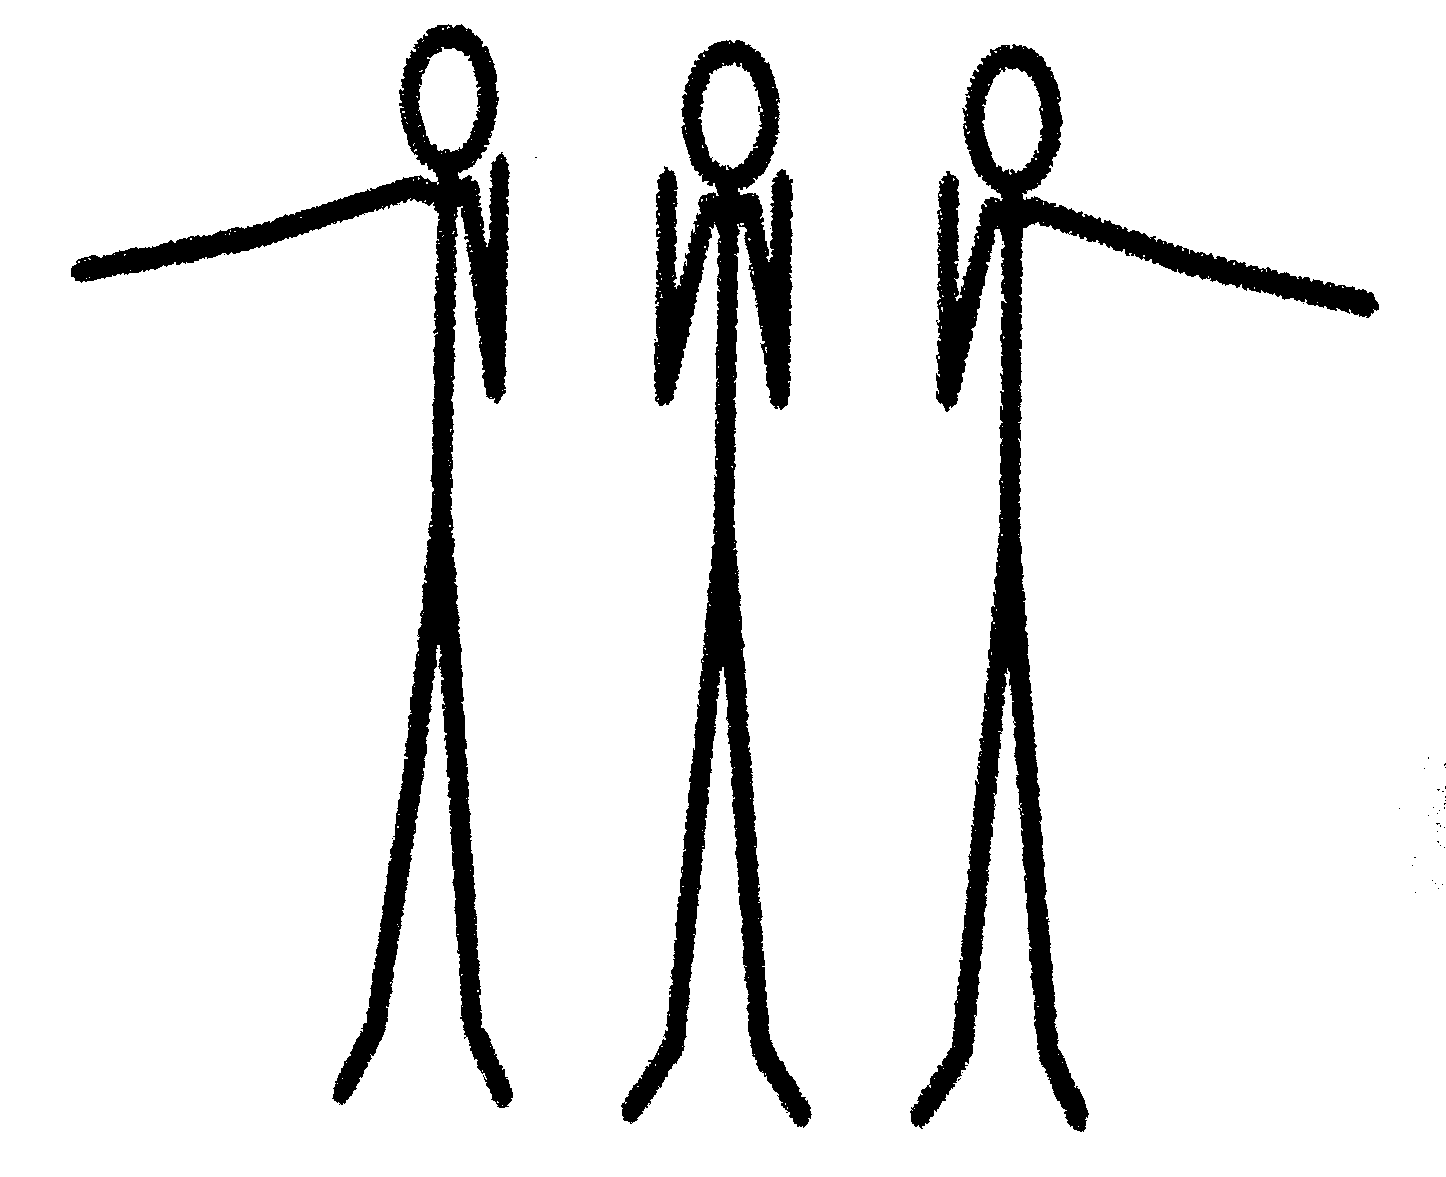
\includegraphics[width=\linewidth]{ExerciseW.png}

\column{.3\textwidth} % Right column and width
The \structure{exhilaration of happiness and amity}.

\vspace{5mm}
\structure{Relaxes the shoulders and neck and harmonizes the breath}.
\column{.24\textwidth} % Right column and width

\includegraphics[width=\linewidth]{RuneW.png}
\end{columns}

\end{frame}
%------------------------------------------------------------
%------------------------------------------------------------








